%%%%%%%%%%%%%%%%%%%%%%%%%%%%%%%%%%%%%%%%%
% Focus Beamer Presentation
% LaTeX Template
% Version 1.0 (8/8/18)
%
% This template has been downloaded from:
% http://www.LaTeXTemplates.com
%
% Original author:
% Pasquale Africa (https://github.com/elauksap/focus-beamertheme) with modifications by 
% Vel (vel@LaTeXTemplates.com)
%
% Template license:
% GNU GPL v3.0 License
%
% Important note:
% The bibliography/references need to be compiled with bibtex.
%
%%%%%%%%%%%%%%%%%%%%%%%%%%%%%%%%%%%%%%%%%

%----------------------------------------------------------------------------------------
%	PACKAGES AND OTHER DOCUMENT CONFIGURATIONS
%----------------------------------------------------------------------------------------

\documentclass{beamer}
\usetheme{Berlin}
\setbeameroption{hide notes} % Only slides
%\setbeameroption{show only notes} % Only notes
%\setbeameroption{show notes on second screen=right}

%\usetheme{focus} % Use the Focus theme supplied with the template
% Add option [numbering=none] to disable the footer progress bar
% Add option [numbering=fullbar] to show the footer progress bar as always full with a slide count

% Uncomment to enable the ice-blue theme
\definecolor{main}{RGB}{92, 138, 168}
\definecolor{background}{RGB}{240, 247, 255}

%------------------------------------------------
\usepackage[utf8]{inputenc}
\usepackage{booktabs} % Required for better table rules
\usepackage{tikz}
\usepackage{quiver}
\usefonttheme{professionalfonts}
\setbeamerfont{bibliography item}{size=\footnotesize}
\setbeamerfont{bibliography entry author}{size=\footnotesize}
\setbeamerfont{bibliography entry title}{size=\footnotesize}
\setbeamerfont{bibliography entry location}{size=\footnotesize}
\setbeamerfont{bibliography entry note}{size=\footnotesize}

\newcommand{\R}{\mathbb{R}}
\newcommand{\Q}{\mathbb{Q}}
\newcommand{\C}{\mathbb{C}}
\newcommand{\Z}{\mathbb{Z}}
\newcommand{\N}{\mathbb{N}}
\newcommand{\F}{\mathbb{F}}
\newcommand{\Hom}{{\mathrm{Hom}}}
\newcommand{\image}{{\mathrm{Im}}}
\newcommand{\kernel}{{\mathrm{Ker}}}
\newcommand{\coker}{{\mathrm{coker}}}
\DeclareMathOperator*{\colim}{co{\lim}}
\DeclareMathOperator*{\hocolim}{hoco{\lim}}
\DeclareMathOperator*{\holim}{ho{\lim}}
\newcounter{dummy} \numberwithin{dummy}{section}

\newtheorem{proposition}[dummy]{Proposition}

%----------------------------------------------------------------------------------------
%	 TITLE SLIDE
%----------------------------------------------------------------------------------------

\title{Higher Algebraic K-Theory:\\ A simplicial approach}

\subtitle{}

\author{Bhoris Dhanjal}

%\titlegraphic{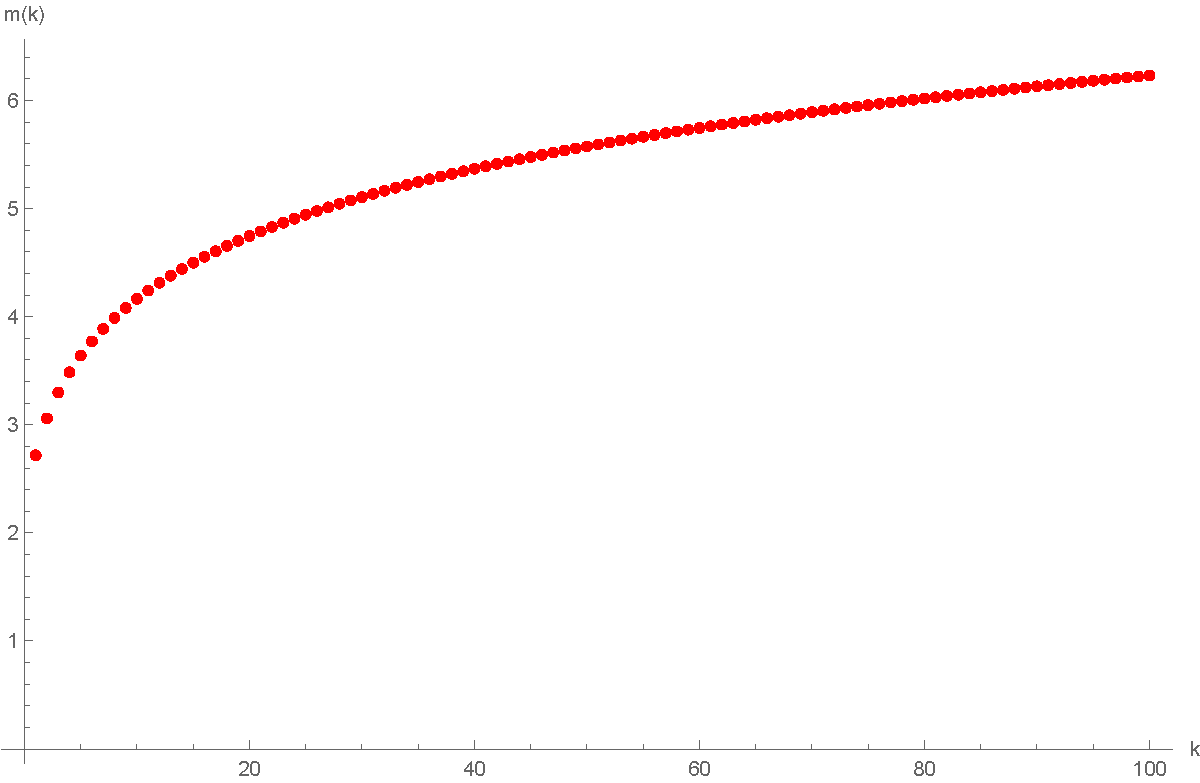
\includegraphics[scale=0.3]{Images/first100rmfc.pdf}} % Optional title page image, comment this line to remove it
\institute{Department of Mathematics,\\ University of Mumbai}

\date{\today}
%------------------------------------------------

\begin{document}

%------------------------------------------------

\begin{frame}
	\maketitle % Automatically created using the information in the commands above
\end{frame}

%----------------------------------------------------------------------------------------
%	 SECTION 1
%----------------------------------------------------------------------------------------



\begin{frame}
	\frametitle{Table of Contents}
	\tableofcontents
\end{frame}

\section{Projective modules}
\begin{frame}{Free modules}
	Recall the definition of a free module.
	\begin{definition}[Free module of rank $n$]
		A module over a ring $A$ is said to be free with rank $n$ if it is isomorphic to a module of the form $A^n$.
	\end{definition}In particular this means that there exists a linearly independent spanning set of the module with $n$ elements.
\end{frame}
\begin{frame}[fragile]{Projective modules}
	\begin{definition}[Projective module]
		A module $P$ is said to be {projective} if it satisfies the following lifting property, every morphism from $P$ to $N$ factors through an epimorphism into $N$. Note that the lift need not be unique.
		\[\begin{tikzcd}
			&& M \\
			\\
			P && N
			\arrow[two heads, from=1-3, to=3-3]
			\arrow[from=3-1, to=3-3]
			\arrow[dashed, from=3-1, to=1-3]
		\end{tikzcd}\]
	\end{definition}

	\note{
		Projective modules were first introduced in 1956 in the influential book Homological Algebra by Henri Cartan and Samuel Eilenberg.
		
		However the primary motiatvation for this definition arises from topology in particular atheorem which we shall prove in the next project called the Serre-Swan theorem.
		
		
		\textbf{Epimorphism: (right cancelative)}In any category $ \mathbf{C} $, an arrow $ f: A \to B $ is called an epimorphism (epic), if for any $ i,j: B \to D $ $ if=jf\implies i=j $.
	\textbf{Monomorphism: }In any category $ \mathbf{C} $, an arrow	$ f: A \to B  $ is called a monomorphism (monic), if for any $ g,h, :C \to A , fg=fh \implies g=h $.
	 A \textbf{split} mono (epi) is an arrow $ m : A \to B$ with a left (right) inverse $ r $. The inverse arrow $ r $ is called the \textbf{retraction}, $ m $ is called a \textit{section} of $ r $ and $ A $ is called a \textbf{retract} of $ B $.
}
\end{frame}
\begin{frame}{Equivalent definition}
		\begin{proposition}[Equivalent definitions of projectivity]\label{projtfae}
		The following are equivalent,
		\begin{enumerate}
			\item $P$ is projective.
			\item For all epimorphisms between $M\twoheadrightarrow N$, the induced map $\Hom(P,g):\mathrm{Hom}(P,M) \to \mathrm{Hom}(P,N)$ sending $f \mapsto g \circ f$ for $g:M \to N$ and $f:P \to M$ is an epimorphism.
			\item For some epimorphism from a free module $F$ to $P$, $\mathrm{Hom}(P,F) \to \mathrm{Hom}(P,P)$ is an epimorphism.
			\item There exists $Q$ s.t. $P \oplus Q$ is free.
			\item Short exact sequences of the form $0 \to A \to B \to P \to 0$ split, i.e. isomorphic to another short exact where middle term is $A \oplus P$.
		\end{enumerate}
		\note{ For point 5 In general any epimorphisms into projective objects split (i.e. have an inverse).
		
		A {chain complex} $(A_\bullet, \varphi_\bullet)$ is a collection of modules over a commutative ring and homomorphisms $\varphi_i: A_i \to A_{i-1}$ such that $\varphi_i \varphi_{i+1}=0$.
		
		
			The {homology} of the complex at $F_i$ is denoted as its $i^{\mathrm{th}}$ homology defined as follows,
		\[ H_iA := \ker \varphi_i/ \mathrm{im} \varphi_{i+1}. \]
		
			A chain complex is said to be {exact} if all its homologies are zero. In particular it is exact at one object if its homology there is zero.
			
			 An exact sequence of the form \[ 0 \to A \to B \to C \to 0 \]
			is referred to as short exact sequence. Note that due to the exactness conditions $A \to B $ is injective and $B \to C$ is surjective.
			
			
		}
	\end{proposition}
\end{frame}
\begin{frame}{Properties of projective modules}
		A projective module is weaker than a free module.
		\begin{lemma}[Free modules are projective]
		\end{lemma}
		\note{Since it is its own summand consider summing with a trivial zero module.
		
		Further flat weaker than projective. (Flat N if tensoring by N defines an exact functor R-mod to R-mod)
		
		For a short exact sequence $$0 \to A \xrightarrow{f} B \xrightarrow{g} C \to 0$$ the following are equivalent:
		\begin{enumerate}
			\item The sequence splits, i.e. $B \cong A \oplus C.$
			\item Left split: There is a morphism $h:B \to A $, such that $hf=1_A$.
			\item Right split: There is a module morphism $i: C \to B $ such that $gi=1_C$.
			\end{enumerate}}
		\begin{example}[Projective modules are not always free]
			Let $R,S $ be two non-trivial commutative rings with unity, consider $R \oplus S$ as a (free) module over itself. Consider $R \oplus \{0\}$ as a submodule of $R \oplus S$, it is projective as it is a direct summand of $R \oplus S$. However, it cannot be free as $(R \oplus \{0\})^n \not \cong R\oplus S $ for any $n$.
		\end{example}
\end{frame}
\begin{frame}{Definitions}
		\begin{definition}[Stably isomorphic]\label{stabiso}
		Two $A-$modules $M,N$ are said to be stably isomorphic if there exists $r$ such that $M \oplus A^r \cong N \oplus A^r$.
	\end{definition}
	\begin{definition}[Stably free module]\label{stabfree}
		An $A$ module $M$ is stably free if there exists a finitely generated free module $F$ such that $M \oplus F$ is free, i.e. if $M$ is stably isomorphic to a finitely generated free $A$ module.
	\end{definition}
	\begin{itemize}
		\item Projective modules over local rings are free.
		\item Projective finitely generated modules over principal ideal domains are free.
	\end{itemize}
\end{frame}

\section{$K_0$ of a ring}
\begin{frame}{Definition of a monoid}
	\begin{definition}[Monoid]
			A monoid is an algebraic object consisting of a set of symbols $A$ with a associative binary operation $+$ and an identity element $e$ (where $a+e=e+a=a$ for all $a \in A$).
	\end{definition}
\begin{example}[Commutative monoid] The natural numbers $\N$ with usual addition $+$.
\end{example}
\begin{example}[Non-commutative monoid]
	Square matrices of size $n$ over some ring $A$ along with matrix multiplication.
\end{example}
\end{frame}

\begin{frame}{Group completion of a commutative monoid}
	We begin with a commutative monoid $A$ to complete it into a group we formally add inverses for each symbol $[a]\in A$. Consider the free group on the set of symbols in the monoid labelled as $F(A)$. Now quotient away all the nontrivial monoidal relations $F(A)/\sim $ where $[a+b]\sim [a]+[b] \sim [b]+[a] \sim [b+a]$. 
	
	This gives us the group completion of a monoid, i.e. the smallest group which has $A$ as a submonoid.
	
	\note{In the noncommutative monoid case such a construction is sometimes referred to as a universal enveloping group of the monoid.}
\end{frame}



\begin{frame}{Group competition of the naturals}
	
		The group completion of the natural numbers $\N$ is $\Z$. Following the group completion procedure as described above we obtain a formal inverse symbol $[b]$ for each symbol $[a] \in \N $, i.e. a symbol $[b]$ such that $[b]+[a]=[a]+[b]=[0]$ for all $[a] \in \N$, but note that this is naturally isomorphic to $\Z $ as $[b] \mapsto [-a]$.

\end{frame}

\begin{frame}{Definition of $K_0$}
\begin{definition}[$K_0$ of a monoid (Group completion functor)]
	For a commutative monoid $A$, the group completion of $A$ is denoted as $K_0(A).$
\end{definition}
\begin{definition}[$K_0$ for a ring $A$]
	Consider the isomorphism classes of finitely generated projective modules over $A$ denoted as $\mathrm{Proj}(A)$. This forms a commutative monoid so $K_0(A)$ is defined as $K_0(\mathrm{Proj}(A))$.
\end{definition}

\note{Since direct sum of projectives is projective converse also true if direct sum projective then summands are projective, isomorphism classes make it a set else its not a set (?)}


\end{frame}

\begin{frame}{Eilenberg swindle}
	\note{This is also used to show that for projective P there is free F such that $P \oplus F \cong F$. Choose $Q$ such that $P \oplus Q$ free and consider $F$ as $F = B \oplus A \oplus B \oplus A \cdots $. Then $A \oplus F \cong F$}

	The reason we require the caveat of finitely generated projective modules instead of simply considering the class of all projective modules is because for the non finitely generated case $K_0(A)$ becomes trivial as we see below.
	\begin{proposition}[Eilenberg Swindle] If we consider $A^\infty$ as a non finitely generated free module over a ring $A$ if $P \oplus Q \cong A^n$ then \[ P \oplus A^\infty \cong P \oplus (Q \oplus P) \oplus (Q \oplus P) \oplus \dots \cong (P \oplus Q) \oplus (P \oplus Q) \oplus \dots \cong A^\infty \] but this relation would imply $[P]=0 $ for all projectives. 
	\end{proposition}
\end{frame}
\begin{frame}[allowframebreaks]{$K_0$ for common algebraic objects}
	\begin{proposition}\label{k0pidisZ}
		If $A$ is a field/division ring/local ring/principal ideal domain then $K_0(A)\cong\Z$.
	\end{proposition}

		For fields and division rings this is true due to all finitely generated modules being free, i.e. having a basis. We prove this directly for division rings for simplicity.
		
		The similar linear algebraic proof extends to division rings for $M$ a module over division ring $A$. Pick a maximally linearly independent subset $B$ by Zorn's lemma. To show \( B \) is a generating set, the argument uses \( B \)'s maximality. If \( m \in M \) then, if $m \in B$ we are done. If $m \not \in B$ then $B \cup \{m\}$ is linearly dependent by maximality of $B$ therefore there exists $a\in A$ such that $am \in \mathrm{span}(B)$ for some $a \neq 0$ and since $a $ is invertible due to $F$ being a division ring we have $m \in \mathrm{span}(B)$.
		Therefore, \( B \) must span \( M \), making it a basis and so $ M \cong A^n$.
		
		Similarly as seen before finitely generated projective modules in a local ring/principal ideal domain are free.
		
		So in each case $\mathrm{Proj}(A) \cong \N$ so its group completion is $\Z.$ 
		
	\note{	Throughout the proof we have implicitly assumed $A$ has the invariant basis property. that $A^n \cong A^m \implies n=m.$}

\end{frame}

\begin{frame}[allowframebreaks]{Computing $K_0$ using idempotents}
	
	We claim that idempotent matrices over $A$ are in a correspondence to finitely generated projective modules over $A$.
	
	For a finitely generated projective module $P$ over $A$, such that $P \oplus Q \cong A^n$ we can define a $R-$module homomorphism which is identity restricted to $P$ and zero else. This is an idempotent element in $M_n(A)$, i.e. $P$ is represented by a $n\times n $ matrix over $A$.
	
	Conversely any idempotent matrix $e \in M_n(A)$ determines a projective. Simply consider the associated module morphism induced by the matrix $e$ and then the image under $e$ is projective, i.e. $eA^n$. This is true because $A \cong eA^n \oplus (1-e)A^n$ \note{Idempotent property is used to show $eA^n \cap (1-e)A^n = 0$ since $e^2=e\implies e(1)$}.
	
	We must make a note of the fact that different idempotent matrices may induce projective modules in the same isomorphism class. This is made precise in the following result.
	
	\begin{proposition}
		If $e, f $ are idempotent matrices over $A$ of possibly different sizes then the associated finitely generated projective modules are isomorphic iff $e,f $ are conjugate over a larger common matrix group of order $r$ (obtained by placing the matrices in the top left corner of a larger 0 matrix).
	\end{proposition}
	
	Consider $GL_n(A) \subset GL_{n+1}(A)$ by placing the $n\times n $ matrix in the top right. In this manner we have a filtered system and we can define $GL(A)= \lim_{\to} GL_i(A)$ as the colimit. Similarly define $M(A)$. Denote the set of idempotent matrices in $M(A)$ as $\mathrm{Idem}(A)$ so we have that the group $GL(A)$ acts on the set $\mathrm{Idem}(A)$ by conjugation.
	
	With the above discussion in mind we now have a alternate description for the monoid $\mathrm{Proj}(A)$ in terms of idempotent matrices. In particular $\mathrm{Proj}(A)$ corresponds to the conjugacy classes of the action of $GL(A)$ on $\mathrm{Idem}(A)$. The monoid operation $e +f$ is the block matrix $\begin{bmatrix}
		e & 0 \\ 0 & f
	\end{bmatrix}. $
	
	\begin{corollary}[Morita invariance of $K_0$]\label{morita}
		Let $A$ be a ring and $n \in \N $ arbitrary. Then $K_0(A) \cong K_0(M_n(A))$.
	\end{corollary}
		Under the realisation $M_n(M_k(A))=M_{nk}(A) $ we can note that the infinite general linear matrices over $M_n(A) $ and $A$ are canonically equivalent, i.e. $GL(M_n(A)) = GL(A)$ in particular their infinite idempotent matrices are also equivalent $\mathrm{Idem}(M_n(A)) = \mathrm{Idem}(A)$. Consequently by the correspondence between idempotent matrices and projective modules their monoid of finitely generated protectives are the same meaning their group completions are isomorphic.
\end{frame}
\begin{frame}{Applications of Morita invariance}
	\begin{corollary}\label{propdirectproductofk0}
		For commutative ring $A$ if $A \cong A_1 \times A_2$ for rings. Then	$K_0(A) \cong K_0(A_1) \times K_0(A_2)$.
	\end{corollary}
	\begin{proof}
		Notice that $GL(A) \cong GL(A_1 \times A_2) \cong GL(A_1) \times GL(A_2)$ and $\mathrm{Idem}(A) \cong \mathrm{Idem}(A_1 \times A_2) \cong \mathrm{Idem}(A_1) \times \mathrm{Idem}(A_2)$.
	\end{proof}
	\begin{corollary}\label{directsystem}
		If $A$ is the direct limit of rings, i.e. $A\cong \lim_{\to i \in I} A_i $ then $K_0(A) \cong \lim_{\to i \in I} K_0(A_i)$.
	\end{corollary}
\end{frame}
\begin{frame}[allowframebreaks]{Simple rings}
	
	\begin{definition}[Simple ring]
		A simple ring is a non-zero ring which have no non-trivial two-sided ideals.
	\end{definition}
	\begin{example}
		A commutative ring is simple iff it is a field.
	\end{example}
	\begin{example}
		All division rings are simple rings.
	\end{example}
	\newpage
	\begin{example}
		Not all division rings are fields consider $M_n(F)$ for some field $F$ not all elements need be invertible.
	\end{example}
	
	A simple module is naturally now any module which is non-zero and has no non-trivial submodules.
	
	\begin{lemma}[Schur's lemma]\label{schurs}
		If $A$ is any ring and $M$ is a simple $R-$module then $\mathrm{End}_A(M)$ is a division ring.
	\end{lemma}
	
\end{frame}
\begin{frame}[allowframebreaks]{Semi-simple rings}
		\begin{definition}[Semisimple ring]
		A ring $A$ is called semisimple if
		\begin{itemize}
			\item $A$ is Artinian with trivial Jacobson ideal. \note{obeys descending chain condition}
			\item $A$ is a finite product of simple Artinian rings.
			\item Every left/right $A-$module is projective.
		\end{itemize}
	\end{definition}
	
\end{frame}
\begin{frame}{Wedderburn-Artin theorem}
	A useful characteristic of semisimple rings is the Wedderburn-Artin theorem.
	
	\begin{theorem}[Wedderburn-Artin]\label{wedart}
		A ring $A$ is semisimple iff it is isomorphic to a direct product of $n_i \times n_i$ matrix rings over division rings $D_i$, i.e. $A \cong \prod_{i=1}^r M_{n_i}(D_i)$ where $D_i =\Hom_A(V_i,V_i), \dim_{D_i}(V_i)=n_i$ for $V_i$ the simple $A$-modules components of $A$.
	\end{theorem}
\end{frame}
\begin{frame}[allowframebreaks]{$K_0$ for a semi-simple ring}
	\begin{lemma}
		Let $A$ be a simple ring then $K_0(A) \cong \Z $.
	\end{lemma}
	\note{The below result is a generalization of Proposition {k0pidisZ} (since every division ring is a simple ring)}
	\begin{proof}
		By Morita invariance \ref{morita} we know that $K_0(A) \cong K_0(M_n(A)) \cong K_0(\mathrm{End}(A)) \cong K_0(D)$ for some division ring $D$. The last isomorphism is due to Schur's lemma \ref{schurs}. Now applying the fact that $K_0$ of a principal ideal domain is $\Z$ we are done.
	\end{proof}
	\begin{theorem}
		If $A$ is a semisimple ring then $K_0(A)\cong \Z^r$.
	\end{theorem}
	\begin{proof}
		Due to Wedderburn-Artin \ref{wedart}, we know $A \cong \prod_{i=1}^r M_{n_i} (D_i)$ now applying Morita invariance \ref{morita}, Corollary \ref{propdirectproductofk0} (the result for $n$ direct sums is obtained via induction).
		$$K_0(A) \cong K_0\left(\prod_{i=1}^r M_{n_i} D_i\right) \cong \prod_{i=1}^r K_0\left( M_{n_i}D_i\right) \cong \prod_{i=1}^r K_0(D_i) \cong \Z^r.$$
	\end{proof}
\end{frame}

\section{Quillen-Suslin}
\begin{frame}{Stable freeness}
		\begin{theorem}[Hilbert-Serre]
		Finitely generated module over $k[x_1,\dots x_n]$ are stably free where $k$ is a principal ideal domain.
	\end{theorem}
	A proof for this uses the fact that $K_0(A) \cong K_0(A[t])$. This is the fundamental theorem of $K_0$ which we prove in the next project on higher K-theory.
\end{frame}

\begin{frame}[allowframebreaks]{Unimodular rows}
		We now introduce an important concept of a unimodular row. This perspective helps greatly simplify the proof of Quillen-Suslin.
	
	\begin{definition}[Unimodular row]
		For a ring $A$, an element of $A^n$ is said to be a unimodular row if its components generate $A$. We denote the set of all unimodular rows of length $n$ in $A$ as $\mathrm{Um}_n(A)$.
	\end{definition}
	
	In particular $v=(v_1, \cdots, v_n) \in \mathrm{Um}_n(A) $ if there exists $a=(a_1, \cdots a_n) \in A^n$ such that $ v \cdot a = v^t a = \sum_{i=1}^n v_i a_i = 1$.
%	\begin{definition}[Unimodular matrix]
%		In general we say an arbitrary matrix over $A$ not necessarily square is unimodular if it is right invertible (i.e. a surjective map).
%	\end{definition}
	Alternatively it can be useful to view a unimodular row as as element of $M_{1 \times n} (A) $ as such it represents a surjective linear map $A^n \to A$, or even an element in $M_{n \times 1}$ in which case it represents a injection from $A \to A^n$.
	
	Recall the definition of a stably free projective module. Based on these definitions we can see that the kernel of the surjective $1 \times n $ matrix $A^n \to A$ (i.e. of a unimodular row) is precisely a stably free projective of the form $\underbrace{P}_{\ker v} \times A \cong A^n$.
	
	
	
	\begin{definition}[Equivalence of unimodular rows]
		For unimodular rows $v,w\in A^n$ we say $v \sim w $ if there exists $ \alpha \in GL_n(A)$ such that $v\alpha =w$.
	\end{definition}
	
	\begin{definition}[Unimodular completion property]
		Given a unimodular row $v=(v_1,\dots v_n) \in A^n$ if we can construct an invertible $n \times n $  matrix with $v$ in the first column we say $v$ has the unimodular completion property.
	\end{definition}
	
	\begin{lemma}
		A unimodular row $v \in A^n$ has the unimodular completion property iff $v \sim (1,0,\dots ,0)$.
	\end{lemma}
	\begin{proof}
		If $v$ can be extended to an invertible matrix $\alpha \in GL_n(A)$ then \[ v\alpha^{-1}  = (1,0,\dots, 0). \]
		Conversely if $\alpha' \in GL_n(A) $ s.t. $v\alpha'=(1,0,\dots,0)$ then $\alpha'^{-1}$ has $v$ in the first column.
	\end{proof}
	\begin{corollary}\label{row-of-inv-mat-unimod}
		Based on the above lemma we can see that naturally any row of an invertible matrix (and column realized as a row of its transpose) is a unimodular row. 
	\end{corollary}
%	\begin{corollary}
%		A projective module $P$ is free iff the unimodular row $v: A^n \to A$ such that $P=\ker v$ is completable to an invertible matrix (since we can adjoin the basis of $P$).
%	\end{corollary}
%	
\end{frame}
\begin{frame}[allowframebreaks]{Horrock's theorem}
		\begin{theorem}[Horrocks' theorem]
		If $(A, \mathfrak{m})$ is a local ring then for any arbitrary unimodular row $v(x)$ in $A[x]^n$ such that one of its component elements has leading coefficient one implies that $v$ has the unimodular completion property. Furthermore, any such $v$ is equivalent to $v(0)$.
	\end{theorem}
	Recall that for a local ring $x \not \in \mathfrak m$ iff $ x  $ is a unit.
	
	When $n=1 $ there is nothing to prove. If $n=2$ by unimodularity of $v(x)$ we have $v_1(x)w_1(x)+v_2(x)w_2(x)=1$ simply consider the matrix
	\[ \begin{bmatrix}
		v_1(x) & -w_2(x)\\
		v_2(x) & w_1(x)
	\end{bmatrix}. \]
	
	We proceed with $n \geq 3$.
	Without loss of generality, we take $v_1(x)$ with degree $d $ among components with leading coefficient $1$ and $\deg v_i < d, $ for $i \neq 1$ by repeated elementary row operations to move the components around. We proceed by inducting on $d$.
	 Our goal to is show that we can choose polynomials $z_1, z_2$ such that $z_1v_1+z_2v_2$ such that adding them onto $v_3$ gives us a polynomial of leading coefficient unit (then reduce to 1) of smaller degree $<d$. Repeating this procedure until $d=0$ would give us a unit component allowing us to cancel out the rest and be left with $v\sim (1,0,\dots,0)$ as expected.
	 
	 The construction and existence of these $z_1,z_2 $ are detailed in the project.
\end{frame}

\begin{frame}[allowframebreaks]{Sketch of proof of Quillen-Suslin}
	We now extend the idea of Horrocks' theorem.
	\begin{lemma}\label{horrocksbutforlocal}
		For an integral domain $A$ and a multiplicative subset $S$ if $v(x) \sim v(0)$ unimodular over $A_S[x]^n $ then there exists $b \in S$ such that \\$v(x+by) \sim v(x) $ over $A[x,y]^n.$
	\end{lemma}
		\begin{lemma}\label{horrocksbuteverything}
		For an integral domain $A$ and $v(x)$ unimodular row in $A[x]^n$ with at least one component having leading coefficient one implies $v(x) \sim v(0)$.
	\end{lemma}
	\begin{theorem}
		For $A=k[x_1, \dots, x_n]$ where $k $ is a principal ideal domain, then $v \sim (1,0,\dots, 0)$ for any unimodular row $v \in A^n$.
	\end{theorem}
	
		\begin{theorem}[Quillen-Suslin]
		Finitely generated projective modules over $A=k[x_1,\dots,x_n]$ where $k$ is a principal ideal domain are free.
	\end{theorem}
	We know such finitely generated projective modules are stably free, and from above we know any unimodular row in $A$ is equivalent to $(1,0,\dots,0)$.
		
		That is to say we wish to prove given a finitely generated projective module $P$ which is stably free, i.e. $P \oplus A^{m_1} \cong A^{m_2}$ then $P$ is free.
		
		When $m_1=1$ this is the split exact sequence (since P is projective see \ref{projtfae}),
		\[ 0 \to A \to A^{m_2}  \to P \to 0 \]
		The injection $A \to A^{m_2}$ is precisely a unimodular row by definition which we know must correspond to the canonical embedding of $1 \mapsto (1,0,\cdots, 0)$.
		So,$$P = \mathrm{im}(A^{m_2} \to P) \cong A^{m_2}/\ker (A^{m_2} \to P) \cong A^{m_2}/\mathrm{im}(A \to A^{m_2}).$$
		Note $A^{m_2}/\mathrm{im}(A \to A^{m_2})$ is free since $\mathrm{im}(A \to A^{m_2})$ is naturally free due to the embedding of the unimodular vector as $v \sim e_1$.
		
		When $m_1 \neq 1$ just take $(P \oplus A^{m_1-1}) \oplus A$.

	
\end{frame}

\section{$K_1$ of a ring}
\begin{frame}{Definition}
		\begin{definition}[Whitehead group for a ring] $K_1$ for a ring $A$ is defined as the abelianization of its infinite general linear group.
		$$K_1:= \frac{GL(A)}{[GL(A):GL(A)]},$$
		Where $GL(A)$ the infinite general linear group is the colimit of $GL_n(A)$ with $GL_{n}$ realized as a subgroup of $GL_{n+1}$ by placing the matrix in the top left corner. 
	\end{definition}
	Note that $[GL(A):GL(A)]$ denotes the derived/commutator subgroup of $GL(A)$, the subgroup generated by all commutators $[g:h]=g^{-1}h^{-1}gh$ for $g,h \in GL(A)$.
\end{frame}
\begin{frame}{Elementary matrices}
	\begin{definition}[Elementary matrices]
		We denote the $n\times n$ elementary matrices as $E_n(A)$ generated by standard elementary matrices of the form $e_{ij}(\lambda) := I_{n}+ \lambda E_{ij} $ where $E_{ij}$ is the matrix with $1$ in the $(i,j)$ entry and zero elsewhere.
	\end{definition}
	\begin{lemma}\label{diag1andprodelementary}
		A nonsingular triangular matrix with $1$'s in the diagonal is a product of standard elementary matrices.
	\end{lemma}
\end{frame}

\begin{frame}[allowframebreaks]{Properties of $K_1$}
	\begin{proposition}\label{whiteheadsimple}
		Let $A$ be a ring and $u$ be a unit in $A$, i.e. $u \in A^\times$. Then,
		\[ {\displaystyle {\begin{bmatrix}u&0\\0&u^{-1}\end{bmatrix}}} \equiv I_2 \mod E_2(A).\]
	\end{proposition}
	\begin{proof}
		${\displaystyle {\begin{bmatrix}u&0\\0&u^{-1}\end{bmatrix}}=e_{21}(u^{-1})e_{12}(1-u)e_{21}(-1)e_{12}(1-u^{-1}).}$
	\end{proof}
	\newpage
	\begin{lemma}[Whitehead]\label{whiteheadmain}
		For $\alpha,\beta \in GL_n(A),$ \[ \begin{bmatrix}
			\alpha \beta & 0 \\ 0 & I_n
		\end{bmatrix} \equiv \begin{bmatrix} \alpha & 0 \\ 0 & \beta
		\end{bmatrix} \equiv \begin{bmatrix}
			\beta \alpha  & 0 \\ 0 & I_n 
		\end{bmatrix} \mod E_{2n} (A).\]
	\end{lemma}
	\begin{proof}
		Let $A=M_n(A)$ and note $E_2(M_n(A) ) \subset E_{2n}(A)$ in Proposition \ref{whiteheadsimple}.
	\end{proof}
	\newpage
	\begin{proposition}
		\( [GL(A):GL(A)]=E(A) .\)
	\end{proposition}
	\begin{proof}
		Using Lemma \ref{whiteheadmain} we can see that \[ \begin{bmatrix}
			\alpha^{-1}\beta^{-1} & 0 \\ 0 & I_n
		\end{bmatrix} \equiv \begin{bmatrix}
			\beta^{-1} \alpha^{-1 } & 0 \\
			0 & 1_n
		\end{bmatrix} \mod E_{2n}(A)\]
		So the derived subgroup of $GL_n(A)$ is contained in $E_{2n}(A)$. Furthermore, every elementary matrix $e_{ij}(\lambda)$ is realized as a commutator since, $e_{ij}(\lambda)=[e_{ik}(1 ), e_{kj} (\lambda)]$.
	\end{proof}	
\end{frame}

\section{Results on linear groups}
\begin{frame}[allowframebreaks]{Suslin's normality theorem}
	We now consider a result due to Suslin about the normality of $E_n(A) $ in $GL_n(A)$. The following Lemma due to Vaserstein will be useful.
	\begin{lemma}[Vaserstein]\label{vasersteinlem}
		Let $\alpha \in M_{m,n} (A)$ and $\beta \in M_{n,m}(A)$ then $I_m+\alpha \beta \in GL_m(A)$ implies that $I_n+\beta \alpha \in GL_n(A)$ and, \[ \begin{bmatrix}
			I_m+\alpha \beta & 0 \\ 0 & (I_n+\beta \alpha)^{-1}
		\end{bmatrix} \in E_{m+n} (A).\] 
	\end{lemma}
	\newpage

		\begin{corollary}\label{corofvaserstein}
		Let $v = (v_1,\ldots,v_n)^t$ and $w = (w_1,\ldots,w_n)^t$ be column vectors in $R^n$ such that $w^tv = 0$, and suppose $w_i = 0$ for some $i \leq n$. Then $I_n + vw^t \in E_n(R)$.
	\end{corollary}
	\newpage
	
	\begin{lemma}\label{kernelf}
		For $v$ unimodular row in $R^n,$ and $f: R^n \to R$ a $R-$ linear map determined by $e_i \mapsto v_i $, where $e_i $ is the standard basis element of $R^n$. We have,
		\[ \ker (f) =\left\{w=(w_1,\cdots w_n)^t \mid \sum_i^n w_i v_i =0\right\} \] and it is generated by elements of the form \( \{ v_j e_i - v_i e_j \} \) for positive $i \leq n$.
	\end{lemma}
	\newpage
	\begin{proposition}\label{finalpropfornormality}
		Let $n \geq 3$. If $v \in R^n$ is unimodular, and $w \in R^n$ such that $w^tv = 0$, then $I_n + vw^t \in E_n(R)$ and this is also true if $w$ is unimodular and $v$ is arbitrary by transposition.
	\end{proposition}
	
	\begin{theorem}[Suslin's Normality theorem]
		For $A$, a commutative ring with unity, $E_n(A)$ normal in $GL_n(A)$ for $n \geq 3$.  \note{There is a counterexample for n=2 given by Cohn}
	\end{theorem}
	
		Since $E_n(R)$ is generated by $e_{ij} (\lambda) $ it suffices to check that $\alpha e_{ij}(\lambda) \alpha^{-1} \in E_n(R)$ for $\alpha \in GL_n(A)$.
		
		Recall from \ref{row-of-inv-mat-unimod} that the columns of $\alpha$ and the rows of $\alpha^{-1}$ are unimodular.
		\[ \alpha e_{ij} (\lambda ) \alpha^{-1}= \alpha(I_n+\lambda E_{ij}) \alpha^{-1} = I_n +\lambda c_i r_j\]
		Where $c_i$ is the $i^\mathrm{th}$ column of $\alpha$ and $r_j$ is the $j^{\mathrm{th}}$ row of $\alpha^{-1}$.
		
		Furthermore since $\alpha^{-1}\alpha =I_n $ implies $r_jc_i=\delta_{ij} $ implies using Proposition \ref{finalpropfornormality} that $\alpha e_{ij}(\lambda) \alpha^{-1} = I_n + \lambda c_i r_j \in E_n(A)$.
\end{frame}


\begin{frame}{Quilen's Local-global theorem and Suslins factorial theorem}
\begin{theorem}[Local-global principle]\label{localglobalprinciple}
	Let $v = (v_1, \dots, v_n) \in \mathrm{Um}_n(A[x])$. If $v(x) \sim v(0)$ over $A_{\mathfrak{m}}[x]$ for all maximal $\mathfrak{m} \in A$, then $v(x) \sim v(0)$ over $A[x]$.
\end{theorem}	
	\begin{theorem}[Suslin's factorial theorem]\label{suslinfactorial}
		Given $(v_0,\dots,v_n) \in \mathrm{Um}_{n+1}(A)$ then $n! | \prod_{i=0}^n m_i$, then $(v_0^{m_1}, \dots, v_n^{m_n}) \in \mathrm{Um}_{n+1}(A).$ 
	\end{theorem}
\end{frame}
\nocite{lam1999lectures}
\nocite{lam2001first}
\nocite{lam2010serre}
\nocite{lang02}
\nocite{matsumura_1987}
\nocite{hairyball}
\nocite{rosenberg1995algebraic}
\nocite{suslin1977}
\nocite{suslin1982}
\nocite{weibel2013k}
%------------------------------------------------
\section{References}
\begin{frame}[allowframebreaks]
        \frametitle{References}
        
        \bibliographystyle{unsrt}
    \tiny{\bibliography{references.bib}}
\end{frame}
%------------------------------------------------
\begin{frame}
    \textbf{\Huge{Thanks for listening}}
\end{frame}
%------------------------------------------------


\end{document}
